
\chapter{Coordinate Frames}

%-------------------------------------------------------------
\section{Introduction}
%-------------------------------------------------------------

A key requirement in robotics programming is keeping track of the
positions and velocities of objects in space.  For example, consider
the situation in Figure \ref{fig:robot_w_inset}.  This robot has been
programmed to find the blue teapot and report its position to a remote
user.  The robot's vision system has detected the teapot directly in
front of the camera at a distance of 1 meter.

\begin{figure}
\begin{center}
\includegraphics[]{frames/figs/robot_w_inset.png}
\end{center}
\caption{This robot has located a teapot and must report the location
  to a user.  The inset image shows the view from the robot's camera.}
\label{fig:robot_w_inset}
\end{figure}

In this situation it would not be very helpful to report to the user
that the teapot has been located \texttt{ONE METER IN FRONT OF MY
  CAMERA}.  Presumably, the user wants to know where \emph{in the
  room} the teapot is located. Providing this information requires us
to know each of the following:
\begin{enumerate}
\item{The position of the teapot relative to the camera. }
\item{The position and orientation of the camera relative to the base
  of the robot.}
\item{The position of the robot in the room.}
\end{enumerate}

Determining items 1 and 3 may be challenging problems on their own,
but for now, we will assume that we have access to this information.
The goal in this chapter is to develop a framework for representing
these relative locations and using that information to translate
coordinates from one frame of reference to another.  In this case,
from a frame of reference defined by the position of the camera
(\texttt{THE TEAPOT IS ONE METER IN FRONT OF MY CAMERA}), to a fixed
frame of reference defined relative to the room (\texttt{THE TEAPOT IS
  NEAR THE SOUTH-WEST CORNER OF THE ROOM}).

%-------------------------------------------------------------
\section{Conventions}
%-------------------------------------------------------------

As a first step we need to establish some conventions for describing
locations and orientations in three dimensions.

\begin{figure}
\begin{center}
\begin{tikzpicture}[x=.75cm,y=.75cm]
\draw[thick,->] (-.1,0) -- (3,0) node[anchor=north ] {$x$};
\draw[thick,->] (0,-.1) -- (0,3) node[anchor=east ] {$y$};
\draw[thick] (1.5,-1)  node[anchor=north ] {a}
;

    \foreach \x in {1, 2}
        \draw [](\x,1pt) -- (\x,-3pt)
            node[anchor=north] {$\x$};
    \foreach \y in {1, 2}
        \draw (1pt,\y) -- (-3pt,\y) node[anchor=east] {$\y$};

\end{tikzpicture}
\hspace{.75in}
\begin{tikzpicture}[x=.75cm,y=.75cm]
\draw[thick,->] (-.1,3) -- (3,3) node[anchor=south ] {$x$};
\draw[thick,->] (0,3.1) -- (0,0) node[anchor=east ] {$y$};
\draw[thick] (1.5,-1)  node[anchor=north ] {b};


    \foreach \x in {1, 2}
        \draw []($(\x,3pt)+(0,3)$) node[anchor=south] {$\x$} -- ($(\x, -1pt) +(0,3)$);
    \foreach \y in {2,1}
        \draw (1pt,3-\y) -- (-3pt,3-\y) node[anchor=east] {$\y$};

\end{tikzpicture}
\end{center}
\caption{There are several ways we can draw two-dimensional coordinate systems.  a.  The origin is drawn in the lower-left corner. b. the origin is drawn in the upper-left.}
\label{fig:two_d_coordinates}
\end{figure}


You certainly have experience working with two-dimensional coordinate
systems like the one illustrated in Figure
\ref{fig:two_d_coordinates}a.  This figure follows the common
convention of placing the origin is at the lower-left with the
positive x-axis draw horizontally and the positive y-axis drawn
vertically.

It is possible to draw this coordinate system differently. For
example, the convention when working with coordinates on a computer
screen is to place the origin at the upper-left corner as shown in
Figure \ref{fig:two_d_coordinates}b.

In a sense, Figures \ref{fig:two_d_coordinates}a and
\ref{fig:two_d_coordinates}b are the same coordinate system drawn in
two different ways.  You can imagine picking up the axes in Figure
\ref{fig:two_d_coordinates}a, flipping them over and placing them back
on top of the axes in Figure \ref{fig:two_d_coordinates}b so that the
axes are aligned.


\begin{figure}
\begin{center}

\tdplotsetmaincoords{76}{243}
\begin{tikzpicture}[tdplot_main_coords]

\draw[thick,->] node[inner sep=0pt] (hand) at  (-.3,-.2,0) {\includegraphics[width=.15\textwidth]{frames/figs/left_hand_gray.png}};
%\draw[thick,->] (-2.7,0,0) -- (-3.95,0,0) node[anchor=north east]{$y$};
%\draw[thick,->] (0,-1.55,0) -- (0,-2.8,0) node[anchor=north west]{$x$};
%\draw[thick,->] (0,0,1.1) -- (0,0,2.35) node[anchor=south]{$z$};
\draw[thick,->] (0,0,0) -- (-3.,0,0) node[anchor=north east]{$y$};
\draw[thick,->] (0,0,0) -- (0,-3.,0) node[anchor=north west]{$x$};
\draw[thick,->] (0,0,0) -- (0,0,3.) node[anchor=south]{$z$};
\end{tikzpicture}
\hspace{1in}
\tdplotsetmaincoords{74}{210}
\begin{tikzpicture}[tdplot_main_coords]

\draw[thick,->] node[inner sep=0pt] (hand) at  (.3,0,-.1) {\includegraphics[width=.15\textwidth]{frames/figs/right_hand_gray.png}};
%\draw[thick,->] (1.45,0,0) -- (2.95,0,0) node[anchor=north east]{$x$};
%\draw[thick,->] (0,2.25,0) -- (0,3.5,0) node[anchor=north west]{$y$};
%\draw[thick,->] (0,0,1.2) -- (0,0,2.45) node[anchor=south]{$z$};
\draw[thick,->] (0,0,0) -- (3,0,0) node[anchor=north east]{$x$};
\draw[thick,->] (0,0,0) -- (0,3,0) node[anchor=north west]{$y$};
\draw[thick,->] (0,0,0) -- (0,0,3) node[anchor=south]{$z$};
\end{tikzpicture}
\end{center}
\caption{Left and right-handed coordinate systems.}
\label{fig:left_right_coordinates}
\end{figure}


The situation is different in three dimensions.  Depending on how the
axes are arranged we can end up with one of two fundamentally
incompatible coordinate systems as illustrated in Figure
\ref{fig:left_right_coordinates}.  The coordinate system on the left
is referred to as a \vocab{left-handed coordinate system}, while the one on
the right is a \vocab{right-handed coordinate system}.  In a right-handed
coordinate system we determine the direction of the $z$-axis by aiming
the pointer finger of the right hand along the positive $x$-axis and
curling our palm toward the positive $y$-axis.  The thumb will then
point in the direction of positive $z$.  For a left-handed coordinate
system we follow the same procedure using the left hand.

There is no way to rotate these two coordinate systems so that they
align.  They represent two incompatible ways of representing
three-dimensional coordinates.  This means that whenever we provide
coordinates in three dimensions we must specify whether we are using a
left-handed or right-handed system.  There is no universal convention
for which should be used, but right-handed systems are more common in
robotics.  All of the examples in this book will assume right-handed
coordinate systems.

%x forward, y left, z up
\begin{figure}
\begin{center}
\tdplotsetmaincoords{60}{110}
\begin{tikzpicture}[tdplot_main_coords]

\draw[thick,->] node[inner sep=0pt] (hand) at  (0,.2,0) {\includegraphics[width=.15\textwidth]{frames/figs/right_hand_rotation_small.png}};

\tdplotdrawarc[thick,->,color=blue]{(0,0,1.7)}{0.5}{50}{340}{anchor=west,color=black}{$\;\;+\Theta$}

\draw[thick,->] (0,0,-.06) -- (0,0,2.45) node[anchor=south]{$z$};
\draw[thick] (0,0,-1.3) -- (0,0,-2) node[anchor=south]{};


\end{tikzpicture}
\end{center}
\caption{Right-hand rule for determining the direction of positive
  rotations around an axis.}
\label{fig:right_hand_rotation}
\end{figure}


We also need to establish a convention for describing the direction of
a rotation.  Again, we will follow a right-hand rule.  To determine
the direction of positive rotation around a particular axis we point
the thumb of the right hand along the axis in question.  The fingers
will then curl around the axis in the direction of positive rotation.
This is illustrated in Figure \ref{fig:right_hand_rotation}.



%-------------------------------------------------------------
\section{Poses and Coordinate Frames}
%-------------------------------------------------------------

%http://wiki.ros.org/tf/Overview/Transformations

The position and orientation of an object in space is referred to as
its \vocab{pose}\index{pose}.  Any description of an object's pose
must always be made in relation to some to some \vocab{coordinate
  frame}.  It isn't helpful to know that my teapot is at position (-2,
2.2, 1.6) unless I know where (0, 0, 0) is and which directions the
three axes are pointing.

\begin{figure}
  \includegraphics[]{frames/figs/frames.png}
  \hspace{.5in}
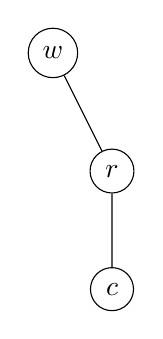
\begin{tikzpicture}
\node[circle,draw](z){$w$}
  child[missing]{}
  child{
    node[circle,draw]{$r$} child{node[circle,draw] {$c$}} };
\end{tikzpicture}

\caption{Left: three coordinate frames from the teapot scenario
  illustrated in Figure \ref{fig:robot_w_inset}.  Right: tree
  representing the relationship between the three coordinate frames.}

\label{fig:frames}
\end{figure}

In robotics, it is often convenient to keep track of multiple
coordinate frames. Figure \ref{fig:frames}  illustrates three potentially useful
coordinate frames related to the teapot scenario described above.  The
``world'' coordinate frame is indicated with the subscript $w$.  This
coordinate frame is fixed at a known location in space and assumed not
to move over time.  The ``robot'' coordinate frame is indicated with
the subscript $r$.  We can envision this coordinate frame as being
attached to the base of the robot so that the origin of the frame
moves as the robot moves.  In other words, the robot is always located
at (0, 0, 0) in its own coordinate frame.  Similarly, the ``camera''
coordinate frame is attached to the camera.

This figure follows the common convention of drawing the $x$-axis in
red, the $y$-axis in green and the $z$-axis in blue.  In the case of
robots (and many other objects) we have a natural notion of directions
corresponding to ``forward'', ``left'' and ``up''.  Throughout this
book these will correspond to positive $x$, positive $y$ and positive
$z$ respectively.

We can organize these three coordinate frames into a tree structure
with the ``world'' coordinate frame as the root.  Each edge in the
tree represents the pose of a particular coordinate frame relative to
its parent.  Ideally, this tree structure should mirror the physical
connections between the objects involved.  In this case it makes sense
to describe the pose of the camera in the robot's coordinate frame,
because the two are physically attached and the camera is constrained
to move along with the robot.  When the robot moves, it is only
necessary to update the pose of the robot coordinate frame.  The
camera remains stationary relative to the robot.

%% Restricting our graph structure to be a tree prevents ambiguity.  If
%% there were more than one path from the root to a particular node then
%% it would require extra effort to make sure that the two paths are in
%% agreement.

Assuming a connected tree, it will be possible to translate a point
between any two coordinate frames.  For example, given the coordinates
of the teapot in the camera coordinate frame, we can determine its
coordinates in the robot coordinate frame, and then in the room
coordinate frame.  In order to accomplish this we need to specify how
poses are represented.  We also need a mechanism for converting from
parent to child coordinate frames and vise-versa.



\subsection{Translations}
\label{sec:tranlations}
Recall that the pose of an object (or a coordinate frame) includes
both its position and orientation relative to the parent coordinate
frame.  Representing the position is straightforward.  Three numbers
may be used to represent a translation of the object along each of the
three axes of the parent coordinate frame.


\begin{figure}
\begin{center}
\includegraphics[]{frames/figs/translation.png}
\end{center}
\caption{Two coordinate frames separated by a simple translation. The
  parent frame is labeled $p$, the child frame is labeled $c$. }
\label{fig:translation}
\end{figure}

Figure \ref{fig:translation} shows two coordinate frames separated by
a simple translation.  In this example, the child coordinate frame
is located at position (1.5, 1.0, .5) in the parent coordinate
frame.

We will use subscripts to indicate the coordinate
frame associated with a point or pose.  For example,
$(0, 0, .5)_c$, refers to the point $(0, 0, .5)$
in the child coordinate frame.

When coordinate frames are separated by a pure translation
transforming points between frames is straightforward: we only need to
add or subtract the three coordinate offsets.  For example, the point
$(0, 0, .5)_c$ is located at $(0 + 1.5, 0 + 1.0, .5 + .5) =
(1.5, 1.0, .5)$ in the parent coordinate frame.  Moving from the
parent to the child requies us to subtract instead of add: $(0, 0,
.5)_p$ is located at $(-1.5, -1.0, 0)$ in the child frame.


\subsection{Euler Angles}
\label{sec:euler}

Specifying orientation in three dimensions is more complicated than
specifying position.  There are several approaches, each with its own
strengths and weaknesses.  \vocab{Euler angles} are probably the most
intuitive representation. Figure \ref{fig:euler} illustrates the basic
idea.  Orientation is expressed as a sequence of three rotations
around the three coordinate axes.  These three rotations are
traditionally referred to as \vocab{roll}, \vocab{pitch} and \vocab{yaw}.

\begin{figure}
\begin{center}
\tdplotsetmaincoords{60}{130}
\begin{tikzpicture}[tdplot_main_coords]

\draw[thick,->] node[inner sep=0pt] (hand) at  (0,0,0) {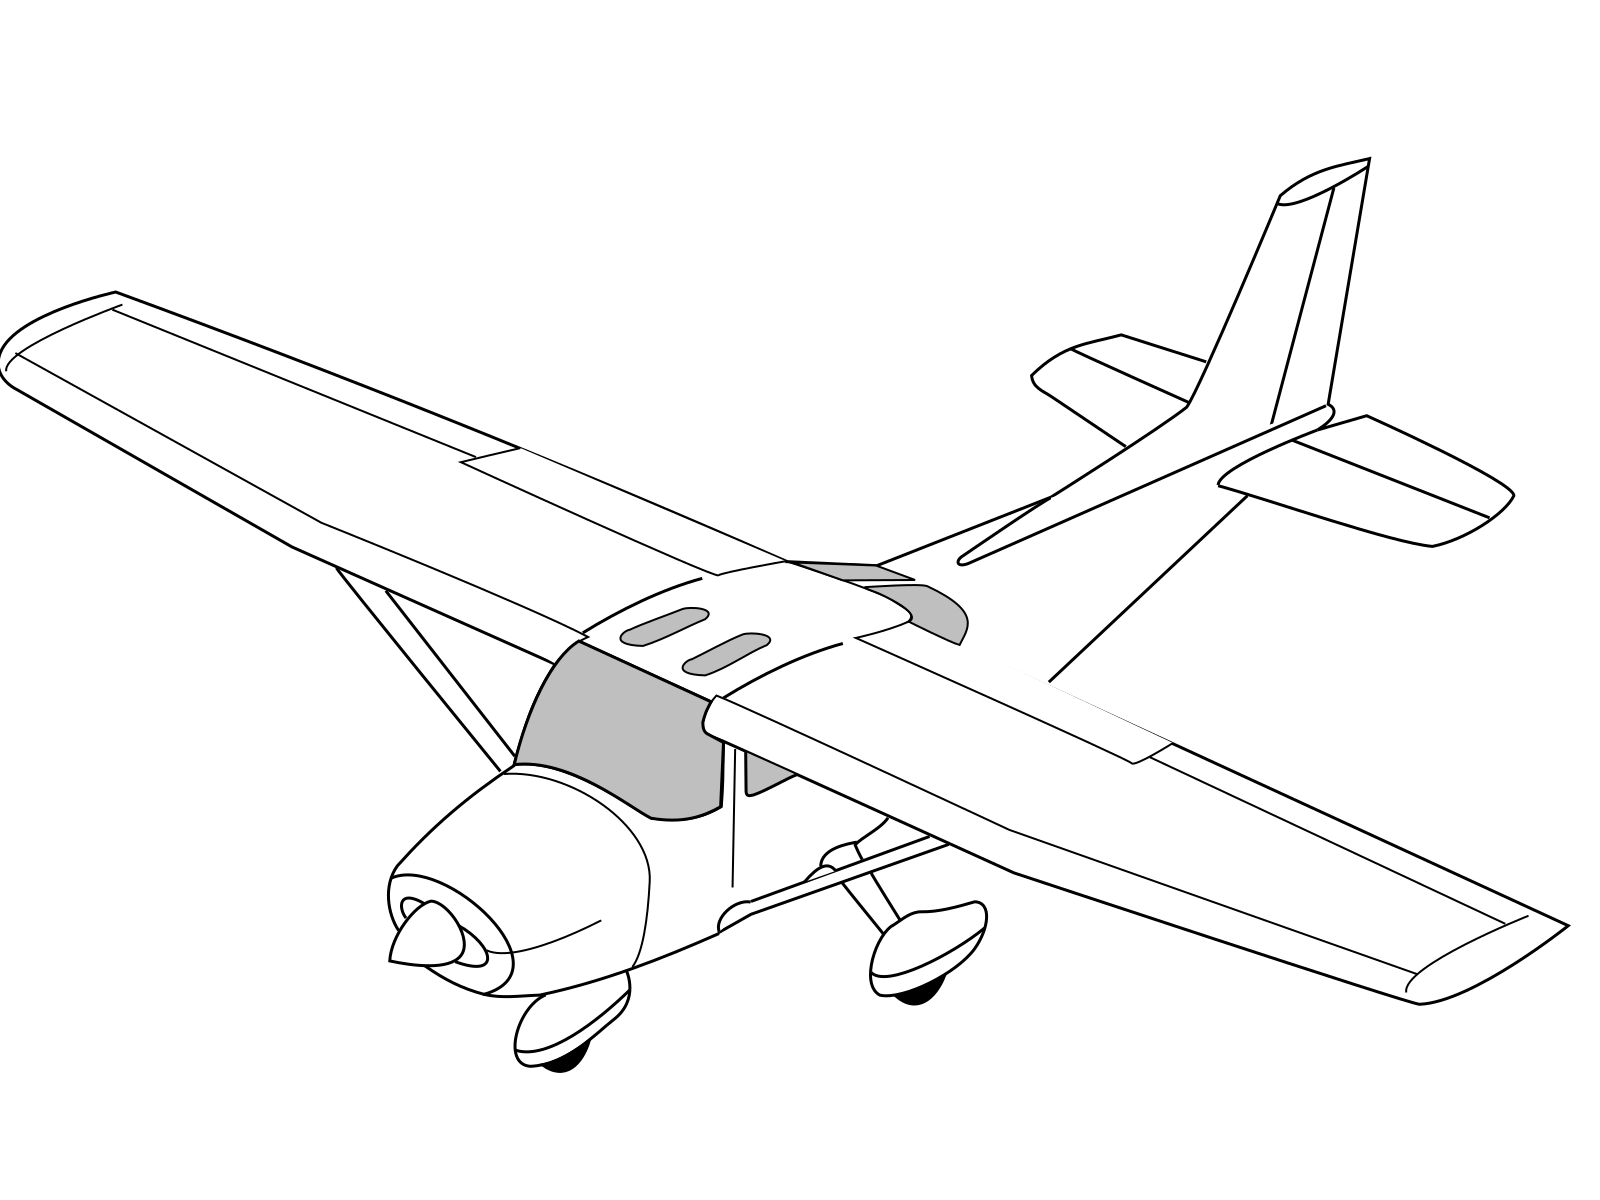
\includegraphics[width=.15\textwidth]{frames/figs/airplane-297578.pdf}};

\draw[thick,->] (0,0,0) -- (3,0,0) node[anchor=north east]{$x$};
\draw[thick,->] (0,0,0) -- (0,3,0) node[anchor=north west]{$y$};
\draw[thick,->] (0,0,0) -- (0,0,3) node[anchor=south]{$z$};

\tdplotdrawarc[thick,->,color=blue,inner sep=10]{(0,0,1.7)}{0.3}{50}{340}{anchor=west,color=black}{yaw}

\tdplotsetrotatedcoords{ 0 }{ 90 }{ 0 }
\tdplotdrawarc[thick,->,color=blue,tdplot_rotated_coords,inner sep=10]{(0,0,1.7)}{0.3}{50}{340}{anchor=east,color=black}{roll}

\tdplotsetrotatedcoords{90  }{ 90}{ 0 }
\tdplotdrawarc[thick,->,color=blue,tdplot_rotated_coords,inner sep=10]{(0,0,1.7)}{0.3}{50}{340}{anchor=west,color=black}{pitch}
\end{tikzpicture}


\end{center}
\caption{Euler angles.}
\label{fig:euler}
\end{figure}


When working with Euler angles it is necessary to specify the order
that the rotations will be applied: a $90^o$ rotation around the
$x$-axis followed by a $90^o$ rotation around the $y$-axis does
\emph{not} result in the same orientaion as the same rotations applied
in the opposite order.  There are, in fact, \emph{twelve} valid
rotation orderings: xyz, yzx, zxy, xzy, zyx, yxz, zxz, xyx, yzy, zyz,
xzx, and yxy.


\begin{figure}
\begin{center}

\begin{tikzpicture}
\node[inner sep=0pt] (e0) at (0,5.0)
    {\includegraphics{frames/figs/euler_static_0.png}};
\node[inner sep=0pt] (e1) at (6.0,5.0)
    {\includegraphics{frames/figs/euler_static_1.png}};
\node[inner sep=0pt] (e2) at (0,0)
    {\includegraphics{frames/figs/euler_static_2.png}};
\node[inner sep=0pt] (e3) at (6.0,0)
    {\includegraphics{frames/figs/euler_static_3.png}};
\draw[->,thick,dashed,>=latex,gray] (2,0) -- (3.5,0);
\draw[->,thick,dashed,>=latex,gray] (2,5) -- (3.5,5);
\draw[->,thick,dashed,>=latex,gray] (3.5,3) -- (2,2);
\end{tikzpicture}

\end{center}
\caption{Static}
\label{fig:static_rotations}
\end{figure}


\begin{figure}
\begin{center}

\begin{tikzpicture}

\node[inner sep=0pt] (e0) at (0,5.0)
    {\includegraphics{frames/figs/euler_nonstatic_0.png}};
\node[inner sep=0pt] (e1) at (6.0,5.0)
    {\includegraphics{frames/figs/euler_nonstatic_1.png}};
\node[inner sep=0pt] (e2) at (0,0)
    {\includegraphics{frames/figs/euler_nonstatic_2.png}};
\node[inner sep=0pt] (e3) at (6.0,0)
    {\includegraphics{frames/figs/euler_nonstatic_3.png}};


\draw[->,thick,dashed,>=latex,gray] (2,0) -- (3.5,0);
\draw[->,thick,dashed,>=latex,gray] (2,5) -- (3.5,5);
\draw[->,thick,dashed,>=latex,gray] (3.5,3) -- (2,2);

%\draw[->,thick,dashed,>=latex] (e1.south west) -- (e2.north east);
%\draw[->,thick,dashed,>=latex] (e2.east) -- (e3.west);
\end{tikzpicture}

\end{center}
\caption{Non static}
\label{fig:nonstatic_rotations}
\end{figure}




It is also necessary to specify whether the rotations are relative to
the parent coordinate frame, or whether each rotation is performed
around the axes of a coordinate frame aligned with the earlier
rotations.  These two alternatives are illustrated in Figures
\ref{fig:static_rotations} and \ref{fig:nonstatic_rotations}.  The
first alternative is sometimes referred to as ``static'' or
``extrinsic'' rotations, while the second may be referred to as
``relative'' or ``intrinsic'' rotations.  Combined with the choice of
axis orderings, this means that there are twenty-four possible
conventions for specifying Euler angles.

Euler angles are relatively easy to visualize, but they are
inconvenient to work with from a mathematical point of view.  The key
problem is that the mapping from spatial orientations to Euler angles
is discontinuous: small changes in orientation may cause big jumps in
the required representation.  This can cause difficulties when we need
to smoothly update the orientation of a moving object over time.

\subsection{Axis Angle}

\begin{figure}
\begin{center}

\begin{tikzpicture}

\node[inner sep=0pt] (e2) at (0,0)
    {\includegraphics{frames/figs/euler_nonstatic_0.png}};
\node[inner sep=0pt] (e3) at (6.0,0)
    {\includegraphics{frames/figs/axis_angle.png}};


\draw[->,thick,dashed,>=latex,gray] (2,0) -- (3.5,0);
%\draw[->,thick,dashed,>=latex] (e1.south west) -- (e2.north east);
%\draw[->,thick,dashed,>=latex] (e2.east) -- (e3.west);
\end{tikzpicture}

\end{center}
\caption{Axis-angle representation of orientation.}
\label{fig:axis_angle}
\end{figure}

Euler angles encode an orienation using three rotations around
pre-defined axes.  An alternate approach is to encode an orientation
as a \emph{single} rotation $\Theta$ around an arbitrary unit vector
$[k_x,k_y,k_z]^T$.
%define unit vector?? refer to appendix??
This is referred to as the \vocab{axis-angle} representation.  The
idea is illustrated in Figure \ref{fig:axis_angle}.

\subsection{Quaternions}

Probably the most widely used method for encoding orientation is the
\vocab{quaternion}.  There is a close relationship quaternions and the
axis-angle representation described above.  If $\Theta$ and
$[k_x,k_y,k_z]^T$ describe the axis-angle representation of an
orientation, then the quaternion represetation is a four-tuple $(x,
y, z, w)$ such that:

\begin{align} 
x =&  k_x \sin{\frac{\Theta}{2}}\label{eq:quat1}\\
y =&  k_y \sin{\frac{\Theta}{2}}\label{eq:quat2}\\
z =&  k_z \sin{\frac{\Theta}{2}}\label{eq:quat3}\\
w =& \cos{\frac{\Theta}{2}} \label{eq:quat4}
\end{align}

Notice that the $x$, $y$ and $z$ components point in the same
direction as the original axis of rotation.  A quaternion constructed
according to Equations \ref{eq:quat1}-\ref{eq:quat4} is also referred
to as a unit-quaternion because it has the property that $\sqrt{ x^2 +
  y^2 + z^2 + w^2} = 1$.

Quaternions are \emph{not} particularly intuitive or easy to
interpret. Their popularity is based on the fact that they support
efficient computation and they avoid the troublesome discontinuities
associated with Euler angles.


\subsection{Rotation Matrices}

Until now we have represented spatial coordinates as ordered triples:
$(x, y, z)$. Equivalently, we may think of points in space as
three-dimensional column vectors: $\begin{bmatrix}x& y&
  z\end{bmatrix}^T$.  This view is convenient because certain spatial
  transformations may be accomplished through matrix operations.  In
  particular, any rotation can be encoded as a $3\times3$
  \vocab{rotation matrix}.  Pre-multiplying the matrix by a point will
  have the effect of performing the desired rotation around the
  origin.

The following three matrices correspond to rotations around the $x$,
$y$, $z$ axes respectively:

\begin{samepage}
\begin{equation}
R_x(\Theta) = 
\begin{bmatrix}
1 & 0 & 0 \\
0 & \cos{\Theta} & -\sin{\Theta} \\
0 & \sin{\Theta} & \cos{\Theta} \\
\end{bmatrix}
\end{equation}

\begin{equation}
R_y(\Theta) = 
\begin{bmatrix}
 \cos{\Theta}& 0  & \sin{\Theta} \\
0 & 1 & 0 \\
-\sin{\Theta} & 0  & \cos{\Theta} \\
\end{bmatrix}
\end{equation}

\begin{equation}
R_z(\Theta) = 
\begin{bmatrix}
\cos{\Theta} & -\sin{\Theta} & 0 \\
\sin{\Theta} & \cos{\Theta} & 0 \\
0 & 0 & 1 \\
\end{bmatrix}
\end{equation}
\end{samepage}

Figure \ref{fig:example_matrix} shows the example of rotating the
point $\begin{bmatrix}1& 0& 0\end{bmatrix}^T$ by $90^o$ around the
  $z$-axis.

\begin{figure}
\begin{minipage}{.25\textwidth}
  \includegraphics[]{frames/figs/rot_matrix.png}
  \end{minipage}%
  \begin{minipage}{.75\textwidth}


\begin{align*}
R_z(90^o) \times 
\begin{bmatrix}
1\\
 0\\
 0
\end{bmatrix} &=
\begin{bmatrix}
\cos{90^o} & -\sin{90^o} & 0 \\
\sin{90^o} & \cos{90^o} & 0 \\
0 & 0 & 1 \\
\end{bmatrix}
\times 
\begin{bmatrix}
1\\
 0\\
 0
\end{bmatrix} \\
&=
\begin{bmatrix}
0 & -1 & 0\\
1 & 0 & 0 \\
0 & 0 & 1 \\
\end{bmatrix}\times 
\begin{bmatrix}
1 \\
 0\\
 0
\end{bmatrix}\\
&=
\begin{bmatrix}0\\
 1\\
 0
\end{bmatrix}
\end{align*}
\end{minipage}
\caption{Example rotation}
\label{fig:example_matrix}
\end{figure}



It is possible to represent any orienation as a product of three
rotation matrices around the $x$, $y$ and $z$ axes.  It is
straightforward to convert from an Euler angle representation to the
corresponding rotation matrix.  For static rotations, the three
elementary rotation matrices must be multiplied in the order that the
rotations should be applied.  This means that the rotation matrix that
corresponds to the Euler angle rotations illustrated in Figure
\ref{fig:static_rotations} would be:

\[ R_{static} = R_x(45^o) \times R_y(30^o) \times R_z(75^o)  
\]

For Euler angles represented using relative rotations, the order is
reversed.  The rotation matrix corresponding to Figure
\ref{fig:nonstatic_rotations} would be:

\[ R_{relative} = R_z(75^o) \times R_y(30^o) \times  R_x(45^o) 
\]

The main advantage of rotation matrices is that they provide a
convenient mechasism for composing rotations and for applying
rotations to a point.  The downside is that this is a highly redundant
represenatation.  A $3\times3$ rotation matrix contains 9 values, but
as we saw in Section \ref{sec:euler} three numbers are sufficient to
represent any orientation in a three dimensional space.


\section{References and Further Reading}

Jennifer Kay provides an excellent and very accessible tutorial on
kinematics and coordinate transforms in \parencite{kay2020}.  That
tutorial also describes \vocab{homogeneous coordinates} which provide a
convenient mechanism for combining rotations and translations into a
single matrix product.

A widely used open-source software library for managing coordinate
frames and performing coordinate transforms is tf/tf2
(\url{http://wiki.ros.org/tf2}).  The tf2 library tracks time-stamped
information about the relative positions and orientations of a tree of
coordinate frames and supports efficient transforms between any two
frames. Introducing a time dimension is valuable because robots move
over time and must interact with dynamic environments. The design and
implementation of the tf library is described in \parencite{foote13}.


%% \subsection{Homogenous Transforms}

%% Recall that our goal is to be able to transform points and poses
%% between coordinate frames that are separated from each other through
%% some combination of translations and rotations.  As we saw in Section
%% \ref{sec:tranlations}  transformations are straightforward as long
%% as the coordinate frames are only separated by pure translations.

%% The method of \vocab{homogenous transforms} provides a convenient
%% mechanism for for performing transformations between \emph{any} two
%% coordinate frames.  Any combination of translations and rotations can
%% be be accomplished through a single matrix multiplication.

%% \vocab{Rotation matrices} may be used to 




% Exercises... Which of the following are right-handed?  Which are left-handed?




